%\documentclass[sigconf, authordraft]{acmart}
\documentclass[sigconf]{acmart}

\usepackage{booktabs} % For formal tables


\setcopyright{rightsretained}

% DOI
\acmDOI{10.1145/nnnnnnn.nnnnnnn}

% ISBN
\acmISBN{978-x-xxxx-xxxx-x/YY/MM}

% Conference
\acmConference[GECCO '20]{the Genetic and Evolutionary Computation Conference 2020}{July 8--12, 2020}{Cancun, Mexico}
\acmYear{2020}
\copyrightyear{2020}

%\acmArticle{4}
\acmPrice{15.00}
% \usepackage{cite}
\usepackage{amsmath,amssymb,amsfonts}
\usepackage{algorithmic}
\usepackage{graphicx}
\usepackage{textcomp}
\usepackage{xcolor}
\usepackage{hyperref}

\begin{document}
\SweaveOpts{concordance=TRUE}

<<setup, cache=FALSE,echo=FALSE>>=
suppressPackageStartupMessages({
    library(ggplot2)
    library(ggthemes)
})
@

\title{Moving target defense through evolutionary algorithms}

%%% The submitted version for review should be ANONYMOUS
\author{Ernesto Serrano-Collado}
\affiliation{%
  \institution{University of Granada}
  \city{Granada}
  \country{Spain}
}
\email{info@ernesto.es}

\author{Mario García-Valdez}
\affiliation{%
  \institution{Instituto Tecnológico de Tijuana}
  \city{Tijuana, Baja California}
  \country{Mexico}
}
\email{mario@tectijuana.edu.mx}

\author{Juan-Julián Merelo Guervós}
\affiliation{%
  \institution{University of Granada}
  \city{Granada}
  \country{Spain}}
\email{larst@affiliation.org}

% The default list of authors is too long for headers.
\renewcommand{\shortauthors}{B. Trovato et al.}


%%%%%%%%%%%%%%%%%%%%%%%%%%%%%%%%%%%%%%%%%%%%%%%%%%%%%%%%%%%%%%%%%%%%%%%%%%%%%
\begin{abstract}

Moving target defense is a technique for protecting internet-facing
systems via the creation of a variable attack surface. In the case of
internet servers, it can be achieved via the generation of different
configurations that change the server profile, and that can be
included in a policy of restarting services with new configurations
after a random time and with a random frequency. In this paper we will
present a method based on evolutionary algorithm, that uses
industry-standard practices to score the vulnerability of a server and
is designed to generate multiple configurations with optimized score
in every run of the algorithm. In this paper we will present how this
is achieved via tuning of the evolutionary algorithm with the
challenge of the very costly fitness evaluation that only allows for a
very limited evaluation budget.
\end{abstract}

\begin{CCSXML}
<ccs2012>
<concept>
<concept_id>10002978.10003006.10011634.10011635</concept_id>
<concept_desc>Security and privacy~Vulnerability scanners</concept_desc>
<concept_significance>500</concept_significance>
</concept>
<concept>
<concept_id>10003752.10003809.10003716.10011136.10011797.10011799</concept_id>
<concept_desc>Theory of computation~Evolutionary algorithms</concept_desc>
<concept_significance>500</concept_significance>
</concept>
<concept>
<concept_id>10010520.10010521.10010537.10003100</concept_id>
<concept_desc>Computer systems organization~Cloud computing</concept_desc>
<concept_significance>300</concept_significance>
</concept>
</ccs2012>
\end{CCSXML}

\ccsdesc[500]{Security and privacy~Vulnerability scanners}
\ccsdesc[500]{Theory of computation~Evolutionary algorithms}
\ccsdesc[300]{Computer systems organization~Cloud computing}

\keywords{Security, cyberattacks, performance evaluation, moving
  target defense, evolutionary algorithms, cloud computing, CVSS}

\maketitle


%%%%%%%%%%%%%%%%%%%%%%%%%%%%%%%%%%%%%%%%%%%%%%%%%%%%%%%%%%%%%%%%%%%%%%%%%%%%%
\section{Introduction}

Cybersecurity is a discipline that taps from all corners of computer
science, including optimization in many cases. Many security problems
can be formulated as a search problem, as long as the vulnerability of
a system (along with any other objective we want to achieve, such as
throughput or performance) can be given a fixed score.

Defending targets against attacks includes many different
techniques. Of course, hardening is one of them, and this is a problem
that can effectively be formulated as an optimization one: minimizing
the vulnerability. A hardened objective might still be attacked, as
long as the person attacking is able to profile it and try different
things on it, simultaneously or later on. Avoiding this is the main
objective of the so called Moving Target Defense, or MTD
\cite{moving-target,jajodia2011moving,Cai2016}.

This kind of defense does not specify either the kind of attack, the
service is protecting or the technique, it is a framework to define a
series of policies where the essence is to change the configuration of the
service defended in that way after a random amount of time so that it
creates different traffic and response patterns that make impossible
to identify a node that does a specific service in the network. In
this sense, we have chosen to work on defending web services (or web
sites) by optimizing the configuration of a web server, following the
work of \cite{john_evolutionary_2014}, which was one of the first
evolutionary approaches to this kind of methodology; unlike he did, we
have chosen the {\sf nginx} static web server and proxy, while he
focused on the well known Apache web server. Our chose was motivated
by the fact that nowadays {\sf nginx} is more popular, and still
growing in popularity nowadays.

In our previous papers \cite{erseco:evostar:anon,erseco:cec}, we realized that one of the main challenges
was to define a fitness function that would be able to reflect changes
in the vulnerabilities exposed by the site, even subtle ones. The
fitness function we used seemed reasonable, and was simply based in
counting the number of alerts raised by ZAP. While this is reasonable,
there are several problems with this, but from the point of view of an
evolutionary algorithm with a very limited budget, the main one is
that most changes in the chromosome will not imply a change in the
fitness; most importantly, a change in the severity of a particular
vulnerability will not be counted as such. This paper will be mainly
devoted to examine a new fitness function, that really takes into
account the severity of the vulnerability raised. We will try to prove
that this new fitness function improves the exploitation capabilities
of the algorithm, obtains more secure configurations, and is also able
to obtain many more low-vulnerability {\sf nginx} configurations in a
single run.

Additionally, we have made several piecewise improvements to our
previous system; we have debugged the configuration extensively to
ensure they produced only valid values; at the same time, we have
eliminated invalid values that were introduced originally for testing
purposes. We have also performed an analysis of the vulnerabilities
reported, in order to check what is the actual impact of configuration
changes on them; finally, we have made a small change to the selection
method to increase the variability of individuals that will be used
eventually for the variable configuration.

The rest of the paper is organized as follows: next we will present
the state of the art in evolutionary methods applied to MTD; the next
Section \ref{sec:met} will present the methodology used in this paper,
followed by the experimental results, which we will discuss in Section \ref{sec:met}
finishing with our conclusions and future lines of work.


%%%%%%%%%%%%%%%%%%%%%%%%%%%%%%%%%%%%%%%%%%%%%%%%%%%%%%%%%%%%%%%%%%%%%%%%%%%%%
\section{Methodology, experimental setup and results}
\label{sec:met}

% Maybe rewrite a part of this, expanding if possible - JJ

As in our previous papers \cite{erseco:evostar:anon,erseco:cec}, we have chosen
{\sf nginx}, a  popular static web server, inverse proxy, API gateway
and load balancer; we did that because web is one of the most popular
(and vulnerable) user-facing services, and it has been also used by
John et al. in their work; that way, we can compare our results.

Latest versions
of{\sf nginx} (1.17.x) have more than 700 configuration
directives. As a matter of fact, the performance of {\sf nginx}
servers has been optimized by  evolutionary algorithms recently
\cite{chi2018hybrid}; however, we will be focused mainly in its
vulnerabilities.


These directives affect in different ways the behavior of
the web site (or service) that is behind it, or simply change the
values in the response headers; we will show the ones we will working
with next. The following Subsection \ref{subs:setup}
will outline the setup actually used for running the experiments, and
results will be presented last in Subsection \ref{subs:results}.

\subsection{Description of the attack surface parameters}

From all the parameters used to change the behavior of {\sf nginx}, we
have chosen just fifteen, the same as in out previous papers
\cite{erseco:evostar:anon,erseco:cec}, from where this section is largely taken
and expanded.

The fifteen parameters we have used in this paper is extracted from the DISA STIG recommendations for
hardening webservers based in the CVSS score
\cite{disa20:apache}, and is also similar to the ones that were chosen
by John et al. \cite{john_evolutionary_2014}.
. Most of these values are defined in the original
document as Apache HTTP server configuration values but have a {\sf
nginx} equivalent directive. All configuration parameters used are
{\sf nginx} directives, with nine of them, shown in Table
\ref{table:nginx_directives}, affecting the global behavior of the
server, and six affecting the values of specific HTTP headers (shown
in Table \ref{table:http_headers}), which in turn affect how the
browser receiving the information deals with the pages and the
information contained in them.

\begin{table*}
\centering
\begin{tabular}{|l|l|c|c|}
\hline
\textbf{STIG ID} &\textbf{Directive name}& \textbf{Possible values} &  \textbf{Used in \cite{john_evolutionary_2014}}\\ \hline
V-13730 & worker\_connections            & 512 - 2048 & \\ \hline
V-13726 & keepalive\_timeout             & 10 - 120 & \checkmark \\ \hline
V-13732 & disable\_symlinks              & True/False & \checkmark \\ \hline
V-13735 & autoindex                      & True/False & \checkmark \\ \hline
V-13724 & send\_timeout                  & True/False & \checkmark \\ \hline
V-13738 & large\_client\_header\_buffers & 512 - 2048 & \\ \hline
V-13736 & client\_max\_body\_size        & 512 - 2048 & \\ \hline
V-6724  & server\_tokens                 & True/False & \checkmark \\ \hline
        & gzip                           & True/False & \\ \hline
\end{tabular}
\vspace{3ex}\\
\caption{List of {\sf nginx} HTTP parameters whose value is evolved
  here. Also featured is their presence in
  \cite{john_evolutionary_2014}, although being a different web
  server, the names might be somewhat different.}
 \label{table:nginx_directives}
\end{table*}
%

These are the {\sf nginx} directives that have been used in this paper; their
equivalent STIG ID is shown in Table
\ref{table:nginx_directives} along with the range of values for
generation and ulterior evolution:\begin{itemize}
\item \texttt{worker\_connections}: Maximum number of simultaneous connections that can be opened by an {\sf nginx} process.
\item \texttt{keepalive\_timeout}: Period during which a server-side client
  connection will remain open  before timing out.
\item \texttt{disable\_symlinks}: Restricts opening files that are
  actually symbolic links. When set to off (the default), if  some component of the
  path is a symbolic link the access to that file is denied. An
  additional value, {\tt if\_not\_owner}, is not considered in this study.
\item \texttt{autoindex}: When activated it shows the contents of the directories, otherwise it does not show anything.
\item \texttt{send\_timeout}: sets a value for the waiting time to
  transmit a response to the client; the client will close the
  connection if nothing is received during that time. It is set by
  default to 60s, we will disable it completely (setting it to 0) or
  set it to 1 second.
\item \texttt{large\_client\_header\_buffers}: This directive has two
  values: the number of buffers that will read large client request
  headers, and their size. We just evolve the second number, while the
  first one is set to 4.

\item \texttt{client\_max\_body\_size}: Maximum allowed size of the client request body, specified in the {\tt
  Content-Length} field of the request header. The value will indicate
the maximum number of Megabytes allowed. Over that value, requests
will simply return an error.

\item \texttt{server\_tokens}: Enable or disable the broadcast of the {\sf
  nginx} version on the error pages and in the {\tt Server} response
header. It's on by default, and we admit on or off values, although the
directive can also use a {\em build} value and simply a string.
\item
\texttt{gzip}: This directive enables or disables compression of HTTP
responses. This directive doesn't affect directly the security but
adds entropy to the different generated configurations; it also
affects the performance of the server and its throughput. The
additional parameter {\tt gzip\_min\_length} can be used to limit the
length of files actually compressed.
\end{itemize}

\begin{table}

  \centering
  \caption{Selected list of directives affecting HTTP headers, and the
  values that we are using in this paper. \label{table:http_headers}}


\begin{tabular}{|l|l|}
\hline
\textbf{Header name}           & \textbf{Possible values} \\ \hline
X-Frame-Options                & \shortstack[l]{SAMEORIGIN \\
  ALLOW-FROM \\ DENY} \\ \hline
X-Powered-By                   & \shortstack[l]{PHP/5.3.3 \\ PHP/5.6.8
  \\ PHP/7.2.1 \\ Django2.2 \\ nginx/1.16.0 \\  nginx/1.17.8} \\ \hline
X-Content-Type-Options         & nosniff \\ \hline
Server                         & \shortstack[l]{apache \\ caddy \\ nginx/1.16.0} \\ \hline
X-XSS-Protection	       & \shortstack[l]{0 \\ 1 \\ 1; mode=block} \\ \hline
Content-Security-Policy	       & \shortstack[l]{default-src 'self';\\~frame-ancestors 'self' \\ default-src 'none';\\~frame-ancestors 'none' \\ default-src 'https://*.google.com'} \\ \hline
\end{tabular}

\end{table}
%


With every web page, the HTTP response from the server includes a
number of headers; part of them are automatically added by the server
or have a default value, while others can be configured; these headers
sometimes simply add metadata (like the system date, for instance),
while others have a precise value that is interpreted by the browser,
and thus can have security implications; these headers, which usually
are preceded by {\tt X}, are also usually {\em de facto} standards,
with certain standard values. The ones we have chosen are explained
below, and the values they can take in this research represented in
Table \ref{table:http_headers}. These servers, which do have an
influence in the security, were not used in
\cite{john_evolutionary_2014}.
\begin{itemize}
\item \texttt{X-Frame-Options}: The header that has the same name as this
directive, when set, bans browsers rendering of frame-embedded pages. Web servers can use it to prevent what are called
\textit{clickjacking} attacks on their pages, that is, overlaying a
transparent frame over a site to make users click on the transparent
layer believing they are clicking on the one below. Several values are
possible: only allow if the embedding page belongs to the same site,
for instance, but you can also directly ban it. We have 4 different
options for this, including a value that's intentionally wrong.
\item \texttt{X-Powered-By}: This string should inform of the
name and versions of the application that generated the response, the
webserver or whatever. It
is generally recommended not giving too extensive information in this
header because can reveal details that can facilitate the task of
finding and exploiting security flaws for specific versions just
looking up in an online database. Setting different values do not affect directly to the
security by itself but adds entropy to the generated configurations.
\item
\texttt{X-Content-Type-Options}: This directive controls the operation
of the homonym HTTP response header; when set,  changing the \textit{MIME} types
announced in the `Content-Type' is disabled, which is used to avoid
`MIME type sniffing' attacks; that is, using what browser's heuristics
for detecting MIME type from content to launch a cross-site scripting
attack.
\item
\texttt{server}: This directive is related to the {\tt Server} HTTP
header, which is used to communicate to browsers metadata about the
server software used by the application. This can be as informative or
as misleading as we want; as a matter of fact, it is a good practice
not to give too
extensive information of software versions, but we can cheat the
attacker telling wrong server version info. Doesn't affect directly to
the security but adds entropy to the generated configurations. This
directive, along with {\tt X-Powered-By}, are mainly used for
informative or statistics purposes and do not really change anything
either in content or how it is rendered by the server.
\item
\texttt{X-XSS-Protection}: This directive is used to set the value of
the corresponding HTTP response header; as the rest of these server
directives, it's interpreted by browsers and used by them to avoid
loading pages when they detect reflected cross-site
scripting (XSS) attacks. % Need to clarify this.
\item
\texttt{Content-Security-Policy}: we can set this directive to
different values to avoid the load of certain kind of content. We have
three different values for this directive, allowing content only if
it's loaded from the same page ({\tt self}), loading from nowhere
({\tt none}), or including Google domains (with the directive {\tt https//:*.google.com}), in
this case mainly for user tracking. These values are shown in Table \ref{table:http_headers}
\end{itemize}
%
\begin{figure}[h!tb]

  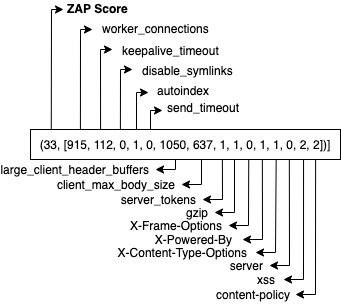
\includegraphics[width=0.95\columnwidth]{chromosome-diagram}
  \caption{Representation of the data structure that stores the
    chromosome, and what the different values represent.}
  \label{fig:chromosome}
\end{figure}
%
This
The problem of optimizing security in configuration is twofold: some
of these directives are security-neutral, and do not actually alter
the security score, they simply add to overall byte-level diversity;
some of them, by themselves, will make a site more secure; in some
other cases, it will be its combination what makes it safer. That is
why a global optimization algorithm is needed to get variable, and
also secure, attack surface. Eventually, a {\sf nginx} configuration
file such as this one will be generated:

\begin{verbatim}
user nginx;
pid /var/run/nginx.pid;
worker_processes 4;
daemon on;
error_log /tmp/nginx-error.log warn;
events {
    worker_connections 667; #
}
http {
    include /etc/nginx/mime.types;
    default_type application/octet-stream;
    access_log /tmp/nginx-access.log;
    sendfile on;
    keepalive_timeout 46; #
    disable_symlinks off; #
    autoindex off; #
    send_timeout 1; #
    large_client_header_buffers 4 804; #
    client_max_body_size 1396736; #
    server_tokens off; #
    gzip off; #
    log_format my_tracking $request_body;
    resolver 8.8.8.8 valid=30s;
    server {
        server_name www.exampletfm.com;
        listen 80;
        error_page 500 502 503 504 /50x.html;
        location ^~ /assets/public/assets/ {
            deny all;
        }
        location ^~ /assets/assets/ {
            deny all;
        }
        location /form {
            access_log /tmp/access.log my_tracking;
        }
        location / {
            root /tester/site/;
            index index.html index.htm;
            add_header X-Frame-Options DENY; #
            add_header X-Powered-By PHP/7.2.1; #
            add_header X-Content-Type-Options nosniff; #
            add_header Server caddy; #
            add_header X-XSS-Protection "1; mode=block"; #
            add_header \\
               Content-Security-Policy "default-src 'self';\\
               frame-ancestors 'self';";#
        }
    }
}
\end{verbatim}

The fifteen parameters that have been generated by the evolutionary
algorithm are marked with a hash mark \# in the block of text
above. The upper block are global
directives, the lower {\tt server} block  affects only the root location, leaving
other subdirectories unaffected.

Not all of these directive actually affect fitness, and thus
vulnerability of the site, and those that do, they create different
kind of vulnerabilities; most of them are about (purported) revelation
of data, but some of them, mainly those related to headers, might
result in some low-level vulnerability.

\subsection{Experimental setup}
\label{subs:setup}

The most important part of the evolutionary algorithm is designing
correctly the fitness function that is going to be tested and used.
A configuration is meaningless without
content behind, and we need to choose what is going to be the
content. As in our previous papers
\cite{erseco:evostar:anon,erseco:cec}, we have used a basic
application with just a few pages and a form, intentionally done that
way so that we can obtain results relatively fast for the new shape of
the algorithm we are testing here.

The setup used for computing this score is exactly the same as before:
standard Docker containers for the juice shop and the ZAP
API were connected together using Docker Compose  with the container
hosting the evolutionary algorithm, which calls from the fitness
function (written in Python) the ZAP library.

For running the Docker containers a set of cloud servers were
orchestrated in Microsoft Azure using standard B2s machine (2 vCPU,
4 GiB of memory) for the 16 population size and standard D2s v3 machine
(2 vCPU, 8 GiB of memory) for the 32 population one. The 16 population
size machine was powered 18 days and the 32 population one was powered
8 days having a total cost of €32.56.

What ZAP does is to run (spider)
over all pages in the site, making different attacks and raising
alerts if they detect any vulnerability. For every vulnerability
found, it raises an alert. In our previous paper we simply used the
number of alerts as a fitness score (to be minimized); while being
adequate for a proof of concept, it does not actually reflect the
state of vulnerability created by the configuration under evaluation,
mainly because these alerts have different nature.

ZAP classifies alerts in four different classes, depending on its
severity: High, Medium, Low and Informational. Of these kind of
vulnerabilities, Informational can be dismissed, since they are simply
notes about some best practice not being followed strictly. For
instance, one such alert could be:

\begin{verbatim}
The response appears to contain suspicious comments
which may help an attacker.
\end{verbatim}

We decided to work with the rest to assign a vulnerability score to
every configuration: Low will be scored with 1, Medium will get 2 as
score, and High will get a 4 score.

This score is to be minimized, but a ``good'' configuration will be
one that does not have any ``Medium''-scored alert.

Evaluation of every configuration is carried out in the following way:\begin{itemize}

\item A new configuration is generated from the evolutionary algorithm
  values and stored in a configuration file with random name. This has
  been introduced in this version, and makes sure that every
  configuration is evaluated only once.

\item This configuration is checked for correctness, and 999 returned
  as score if it's incorrect.
\item The program ensures the previous instance of the server has been
  killed, and starts up the server.
\item ZAP scans the site
\item The program kills the server, checking several times until it's gone

\end{itemize}

Scanning is the part of this process that takes the most time, since
it implies making requests to every single page in the system and
analyzing the response. In this version of the tester we have
increased the number of maximum workers the {\sf nginx} server is able
to process, which might speed it up a bit. Still, a single run takes
several hours, leaving us with just a few possible experiments to
conform, and every one of them with just a few evaluations, much less
that are standard in the industry.

After testing different types of crossover and mutation in our
previous papers \cite{erseco:evostar:anon,erseco:cec}, in this paper
we have used the simple combination of operators we tested in the
previous version, that is, used an  {\em incremental} mutation, that
adds or subtracts one from
current values, and circles back to the opposite end of the range if
these are exceeded; for instance,  the value of {\tt worker\_connections} is
2048 it will become 512 if it's added one. This guarantees that every
mutation will result in a different value of the parameter under
mutation; also, only one randomly chosen value is changed every
time. Additionally, we are using a traditional 2-point crossover that
returns a single chromosome (as opposed to the traditional two),
combining 3 segments, two taken from one parent, one taken from the
other. Also, we are again using 2-tournament selection.

All together, every generation, a reproduction pool of the same size
as the population is created; these are randomly paired,
crossed, obtaining a single result, that is then mutated; this new set
of individuals is evaluated and the result is merged with
the previous population, with just the best ones selected to pass to
the next generation.

A simple, but fundamental change has been added in this paper in the
sorting algorithm used to sort the solutions and select the best
ones: previously, we used the default {\tt sorted} Python function,
which sorts data structures using all the elements of the data
structure sorted. Since we store chromosomes in a list with two
elements, the first of which is the fitness (see Figure \ref{fig:chromosome}, and the second  a list
containing the chromosome, the chromosome itself was included in this
sorting, resulting in selected individuals being similar to each other
as long as their fitness was exactly the same. However, in this paper
we have changed the algorithm to use only the fitness, which is the
first element. When fitness is the same, the chromosomes will be
maintained in the same random order in which they entered the sort
algorithm.


\subsection{Experimental results}
\label{subs:results}

First we will test what are the results with the new fitness function,
as well as the rest of the incremental improvements we made to the
implementation of the evolutionary moving target defense method.
%
\begin{figure}[h!tb]
<<data, cache=FALSE,echo=FALSE>>=
old.fitness.data <- read.csv("results/results-gecco-2020-old-fitness.csv")
old.fitness.data$Experiment <- "Evostar2020"
new.fitness.badsort.data <- read.csv("results/results-gecco-2020.csv")
new.fitness.badsort.data$Experiment <- "Initial sorting"
new.fitness.data <- read.csv("results/results-gecco-2020-ordered.csv")
new.fitness.data$Experiment <- "Current sorting"
data <- rbind (old.fitness.data, new.fitness.badsort.data, new.fitness.data)
ggplot(data,aes(x=Experiment,y=Initial.Avg))+geom_boxplot()+theme_tufte()
@
\caption{Boxplot of initial values of fitness for the EvoStar
  experiment, which used the old fitness and, besides, included
  invalid configuration values, as well as for the new fitness
  function used this paper, with or without any kind of sorting. \label{fig:initial:fitness}}
\end{figure}
One of the changes introduced in this paper, besides the new fitness
function, is the fact that there are no invalid configurations
generated, since all invalid test values have been eliminated from the
chromosome. The previous experiments showed that eventually those
values were eliminated from the population, but they were still
present, adding invalid configurations to the pool of evaluations we
cannot afford. Figure \ref{fig:initial:fitness} shows a boxplot of the
value of the initial fitness; the average for the new fitness
functions, irrespective of sorting used (which has no influence in the
first one). What it shows is that when invalid configurations were
used (and scored at 999) the initial average was too high; the values
now are quite low, and reflect the fact that all configurations are
valid.

As in our previous paper, the best fitness obtained is already present
in an individual in the first generation, so that the evolution
process consists in eventually {\em filling} the population with
individuals with this, highest, fitness. The main difference from
\cite{erseco:evostar:anon,erseco:cec} to this paper is that, in this case,
there will be no chromosome in the last generation with medium
vulnerabilities: all of them, thanks to the new fitness designed, have
low vulnerability, as well as "information-level" vulnerabilities
which are not really considered in this new fitness. As was the case
before, 100\% of all chromosomes share this low vulnerability score.

But the real improvement lays in the use of the new sorting function
to select chromosomes. We represent the average distances in Figure
\ref{fig:md}.
%
\begin{figure}[h!tb]
<<distances, cache=FALSE,echo=FALSE>>=
data.md <- read.csv("results/mutual-distances-averages-entropy.csv")
data.16 = data.md[ data.md$Population == 16, ]
data.32 = data.md[ data.md$Population == 32, ]
ggplot(data.16,aes(x=Experiment,y=Avg.Distance))+ geom_boxplot() + theme_tufte()
ggplot(data.32,aes(x=Experiment,y=Avg.Distance))+ geom_boxplot() + theme_tufte()
@
\caption{Average mutual distance for individuals in the last
  generation for experiments with population = 16 (top) and 32
  (bottom). GECCO labels the ones that use the new sort method, while
  "Sorted" uses the same algorithm, but the whole chromosome, not only
the fitness, is sorted; the data labeled "Evostar" uses the previous
fitness function, sorted in the same way; this one was not tested with
population = 32.}
  \label{fig:md}
\end{figure}
%
The figures clearly show that the per-file average mutual distances
between different individuals have increased, thanks to the simple
change of using a better sorting routine for selection. Average
distances were very similar before that change, and didn't depend on
the type of fitness. All that could be affirmed about the previous set
of solutions was that they were pairwise different; now we can also
affirm that there's a good average distance between them; this
distance is not normalized, however, and could be dominated by a few
components whose range is bigger; this is why we have also computed
the entropy of these distances, charted in Figure
\ref{fig:entropy}. This is the Jenssen-Shannon entropy computed over
the list of pairwise distances.
%
\begin{figure}[h!tb]
<<entropy, cache=FALSE,echo=FALSE>>=
ggplot(data.16,aes(x=Experiment,y=Entropy))+ geom_boxplot() + theme_tufte()
ggplot(data.32,aes(x=Experiment,y=Entropy))+ geom_boxplot() + theme_tufte()
@
\caption{Population-level mutual distance entropy for individuals in the last
  generation for experiments with population = 16 (top) and 32
  (bottom). Labels as above, with GECCO tagging the ones we have
  proposed in this paper.}
  \label{fig:entropy}
\end{figure}
%
Again, entropy is much higher in the new experiment, with this
indicating that how far away a component is going to be from others
has an element of surprise, which is what we are looking for in the
MTD methodology. Still, we need to look at the component-level
entropy, that is, the degree of surprise of a particular element in
the chromosome: see Figure \ref{fig:component:entropy}
%
\begin{figure}[h!tb]
<<component.entropy, cache=FALSE,echo=FALSE>>=
entropy.initial <- read.csv("results/component-entropy-evostar.csv")
entropy.new <- read.csv("results/component-entropy-sorted.csv")
entropy.unsorted <- read.csv("results/component-entropy-gecco.csv")

entropy.initial$Experiment <- "Evostar"
entropy.new$Experiment <- "Sorted"
entropy.unsorted$Experiment <- "GECCO"

entropy.data <- rbind(entropy.initial, entropy.new, entropy.unsorted)

entropy.data$Population <- substr( entropy.data$File, 16, 17 )

ggplot( entropy.data[entropy.data$Population==16,], aes(x=Experiment,y=Entropy)) + geom_boxplot()+ theme_tufte()
ggplot( entropy.data[entropy.data$Population==32,], aes(x=Experiment,y=Entropy)) + geom_boxplot()+ theme_tufte()
@
\caption{Component-level entropy for individuals in the last
  generation for experiments with population = 16 (top) and 32
  (bottom). Labels as above, with GECCO tagging the ones we have
  proposed in this paper.}
  \label{fig:component:entropy}
\end{figure}
%
Once again, added entropy for all components is much higher;
component-wise, there might not be much variation, mainly in those
components that have few values and/or have only some values that
result in low or no vulnerability; the added value, however, is that
this new version of the evolutionary moving target defense framework
is able to generate low-vulnerability, high-diversity, sets of
configurations that can then be used successively in setting
configuration for {\sf nginx} servers, changing them with high frequency.

All the results of experiments, as well as their code and the scripts
needed to generate this data can be found in
% \url{https://github.com/JJ/2020-WCCI-variable-attack-surface}
\url{https://github.com/anonymous/repo}, and can
be reused with a free license.

\section{Conclusions and discussion}
\label{sec:conclusions}

% Write conclusions here
In this paper we have presented an improved evolutionary algorithm
that generates diverse configurations for the {\sf nginx} server, as a
showcase of service-level (and, to a certain point, network-level)
moving target defense. This work has been the result of progressive
code-level refinement of the evolutionary algorithm, as well as an
improvement in the selection strategy and the fitness function.

The main effect of changing the fitness function has been to eliminate
configuration values that created medium-severity vulnerabilities; in
our previous paper \cite{erseco:cec} all vulnerabilities received the
same score, and there could be cases where these stayed in the final
population. But the biggest impact on entropy of the final
configurations has been achieved by changing the sorting
algorithm. While in \cite{erseco:cec} final configurations were
different, parameter-level entropy was small; by making population
selection depend only on fitness and disregard the rest of the
chromosome, parameter-level entropy has received a big boost, which
makes the set of configurations defined by this method better. This
move has had the side effect of keeping diversity high, by introducing
a random element (the order in which individuals were drawn originally
from the population) in the selection procedure, something that was
missing when chromosomes with the same fitness were sorted in
lexicographical order.

What we have not detected in this work is combinations of
configuration values that can create a vulnerability; in general, it's
specific parameter values what make a certain configuration more
secure or not. This, in turn, implies that any hillclimbing approach,
at least for this specific set of parameters selected, valid in the
hardening part of the optimization. However, using an evolutionary
algorithm is still valid because it is able to find secure
configurations at the same time it generates sets of combinations with
a high entropy, as proved in this paper. In general, tricky
combinations of configuration that would make the system insecure
would not be reasonable. Still, a system with many configuration
parameters, as many as 700, will improve security if it totally or in
part is set automatically using optimization algorithms such as this one.

% Future lines of work.
The main challenge of this kind of problem and solving it with
evolutionary algorithms is still evaluation speed, so in the immediate future our focus will be on analyzing the different
parts of the experimental setup so that we can iron out all problems,
and also attain whatever speed ups can be attained with it, so that
evaluation can be faster; for instance, we should try and look at a
way of evaluating several configurations in parallel, and maybe make
the algorithm asynchronous so that it does not have to wait for a full
generation before performing its operations. This is one of the main drawbacks of the algorithm right now,
and although part of it is inherent (it still has to try every single
page of a site), we could try to achieve faster
evaluation by using a different web for generating the configuration
and for deploying the configuration. Using the actual web we are
testing for evolving
configurations can be incredibly time-consuming; the use of surrogates
would speed up evolution, either by creating surrogates of the web
itself or by trying to make parts of the evaluation via surrogates
obtained a deep learning algorithm which, besides, should give us some
insight on the problems created by different features and what predict
insecure configurations just by looking at them, without the need to
put up an actual web site.

In this paper we have also found that the baseline secure
configuration has flaws that do not have anything to do with the
configuration of the web server. We will try to expand the
configuration to the content itself, and also to specific parts of
this content or how it has been generated. We can also extend
evolutionary MTD to other services, whose configurations can be
evolved alongside the web server for more variable attack surfaces, or
even change the web server so that the configuration is even more
difficult to detect. Addinfg multi-objective evolution so that we
improve performance alongside security is also something we intend to
pursue in the future.

%%%%%%%%%%%%%%%%%%%%%%%%%%%%%%%%%%%%%%%%%%%%%%%%%%%%%%%%%%%%%%%%%%%%%%%%%%%%%
\section{Acknowledgements}

This paper has been supported in part by project DeepBio (TIN2017-85727-C4-2-P).

\bibliographystyle{ACM-Reference-Format}
\bibliography{geneura,moving-target}

\end{document}
